\documentclass[12pt, a4paper]{book}

\usepackage[margin=2cm]{geometry}
\usepackage{tikz-cd}
\usepackage{enumitem}
\usepackage{mathtools}
\usepackage{graphicx}
\usepackage{xepersian}
%\settextfont[Script=persian, Scale=1.3]{Vanda}
%\setdigitfont[Scale=1.2]{Vanda}
\settextfont{Yas}
\setdigitfont{Yas}
\begin{document}
\chapter{ترسیم‌های هندسی و استدلال}


\chapter{قضیه‌ی تالس، تشابه و کاربردهای آن}


\chapter{چند ضلعی‌ها}

\section{چند ضلعی‌ها و ویژگی‌هایی از آنها}

\textbf{تعریف:}
n
ضلعی شکلی است شامل 
$\text{n}(3 \geq \text{n})$
پاره‌خط متوالی که:\\
(1 هرپاره‌خطی، دقیقاً دو پاره‌خط دیگر را در نقاط انتهایی خودش قطع کند.\\
(2 هر دو پاره‌خط که در یک انتها مشترک‌اند، روی یک خط نباشند.

\subsection{قطر در چندضلعی‌ها}

در هر
n
ضلعی، هر پاره‌خط را که دو انتهای آن، دو رأس غیرمجاور باشند، قطر می‌نامند.

n
ضلعی 
$\mbox{A}_{1}\mbox{A}_{2} \dots \mbox{A}_{\mbox{n}}$
را در نظر می‌کیریم. از رأس 
$\mbox{A}_{1}$،
n-۱
قطر می‌توان رسم کرد.\\
با توجه به اینکه n رأس داریم، می‌توان گفت تعداد قطرها در n ضلعی با این فرمول به‌دست می‌آید:
\begin{minipage}{2 cm}
	\centering
	$\dfrac{n(n-3)}{2}$
\end{minipage}
\newline

\textbf{مثال:}

تعداد اقطار یک چند ضلعی ۳۵ است. از هر رأس این چندضلعی چند قطر می‌گذرد؟
\begin{flushleft}
$\dfrac{n(n-3)}{2} = 35 \Rightarrow x^2 -3x = 70 \Rightarrow (x-10)(x+7) = 0 \Rightarrow \left\{ \begin{array}{lll}
\fbox{$x =10$} & \mbox{ق‌ق} \\ x = -7 & \mbox{غ‌ق‌ق}
\end{array} \right.$
\end{flushleft}

تعداد اقطار یک چند ضلعی محدب از تعداد اضلاع آن ۴۲تا بیشتر است. این چند ضلعی چند قطر دارد؟
\begin{flushleft}
$\dfrac{n(n-3)}{2} = x+42 \Rightarrow x^2 -3x = 2x +84 \Rightarrow x^2 -5x -84 =0 \Rightarrow (x+7)(x-12) = 0  \Rightarrow \left\{ \begin{array}{lll}
\fbox{$x = 12$} & \mbox{ق‌ق} \\ x = -7 & \mbox{غ‌ق‌ق}
\end{array} \right.$
\end{flushleft}

مجموع تعداد اضلاع و اقطار یک 1 $\!+\!$ n ضلعی نصف اقطار یک 2n ضلعی است.  n چند است؟
\begin{flushleft}
$\dfrac{n+1(n+1-3)}{2} + n+1 = \dfrac{2n(2n-3)}{4} \Rightarrow \dfrac{n^2-n-2}{2}+ n+1 = \dfrac{4n^2-6n}{4} \Rightarrow \dfrac{n^2-n-2+2n+2}{2} = \dfrac{2n^2-3n}{2} \Rightarrow n^2+n = 2n^2 -3n \Rightarrow n^2 -4n = 0 \Rightarrow n(n-4) = 0  \Rightarrow \left\{ \begin{array}{lll}
n =0 & \mbox{غ‌ق‌ق} \\ \fbox{$n = 4$} & \mbox{ق‌ق}
\end{array} \right.$
\end{flushleft}

در یک ۱۰۰ ضلعی محدب تعداد اقطاری که از ۲ رأس غیرمجاور می‌گذرد چند تا است؟
\begin{flushleft}
$100 - 3 = 97 \qquad (2 \times 97) - 1 = 193$
\end{flushleft}

مجموع تعداد اقطار و اضلاع یک چند ضلعی محدب برابر ۱۲۰ است. تعداد اضلاع چند است؟
\begin{flushleft}
$\dfrac{n+1(n+1-3)}{2} + n = 120 \Rightarrow \dfrac{2n^2-3}{2} = 120 \Rightarrow n^2-n=240 \Rightarrow (n-16)(n+15) = 0 \Rightarrow \left\{ \begin{array}{lll}
 \fbox{$n = 16$} & \mbox{ق‌ق} \\ n =-17 & \mbox{غ‌ق‌ق}
\end{array} \right.$
\end{flushleft}

\subsection{چهارضلعی‌های مهم و ویژگی‌هایی  آنها}
\textbf{تعریف:}


	1 -
	متوازی‌الاضلاع چهارضلعی‌ای است که، هر دو ضلع مقابل آن موازی باشند.
	
	2 -
متوازی‌الاضلاع چهارضلعی‌ای است که، هر دو ضلع مقابل آن موازی باشند.

	3 -
	مستطیل چهارضلعی‌ای است که ، همه‌ی زوایای آن قائمه باشند.
	
	4 -
	لوزی چهارضلعی‌ای است که، هر چهارضلع آن هم‌اندازه باشند.
	
	5 -
	مربع چهارضلعی‌ای است که، هر چهار ضلع آن هم‌اندازه و حداقل یک زاویه‌ی آن قائمه باشد.
	\newline

با توجه به تعاریف بالا هر یک از عبارات زیر را نیز می‌توانیم توجیه کنیم: \smallskip\\

\textbf{آ)} مستطیل یک متوازی‌الاضلاع است.

\textbf{ب)} اگر در متوازی‌الاضلاع یکی از زوایا قائمه باشد، مستطیل است.

\textbf{پ)} لوزی یک متوازی‌الضلاع است

\textbf{ت)} مربع یک لوزی، مستطیل و متوازی‌الاضلاع است

\subsection{ویژگی‌هایی از متوازی‌الاضلاع}
متوازی‌الاضلاع چهارضلعی‌ای است که، هر دو ضلع مقابل آن موازی باشند.
\newline

\textbf{قضیه ۱}: هر در متوازی‌الاضلاع هر دو ضلع مقابل هم‌اندازه‌اند.

\begin{minipage}{.7\textwidth}
		\centering فرض: 
		$AB \parallel CD, \; AD \parallel BC$
		\qquad حکم:
		$AB = CD, \; AD = BC$
	\begin{flushleft}
			$ \left. \begin{array}{rll}
		(AB \parallel CD, \, \text{مورب} \, BD ) \rightarrow \widehat{D}_1 = \widehat{B}_1 \\ (AD \parallel BC, \, \text{مورب} \, BD ) \rightarrow \widehat{D}_2 = \widehat{B}_2 \\ AC =AC
		\end{array} \right\} \xrightarrow{\text{زض‌ز}} \triangle ABC \cong  \triangle ADC 
		\Rightarrow AB = CD \, , \, AD = BC$
	\end{flushleft}
\end{minipage}
\begin{minipage}{.28\textwidth}
	\begin{flushleft}
		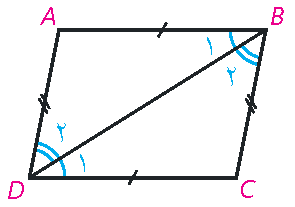
\includegraphics{"Shapes/Fasl - 3/Dars 1/qazie 1.pdf"}
	\end{flushleft}
\end{minipage}
\newline \bigskip \bigskip

\textbf{عکس قضیه ۱}: اگر در یک چهارضلعی، اضلاع مقابل دوبه‌دو هم‌اندازه باشند، چهارضلعی متوازی‌الاضلاع است.

	\begin{minipage}{.73\textwidth}
		\centering
	فرض: 
	$AB = CD, \; AD = BC$
	\qquad حکم:
	$AB \parallel CD, \; AD \parallel BC$
	\begin{flushleft}
		$ \left. \begin{array}{lll}
			AB = CD \\ AD = BC \\ AC = AC
		\end{array} \right\} \xRightarrow{\mbox{زض‌ز}} \triangle ABC \cong  \triangle ADC 
		\Rightarrow \left. \begin{array}{lll}
			 \widehat{A}_1 = \widehat{C}_1 \Rightarrow AB \parallel CD\\ \widehat{A}_2 = \widehat{C}_2 \Rightarrow AD \parallel BC
		\end{array} \right.$
	\end{flushleft}
\end{minipage}
\begin{minipage}{.28\textwidth}
	\begin{flushleft}
		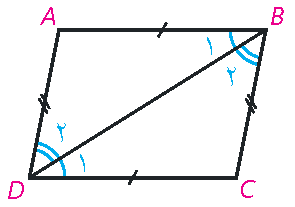
\includegraphics{"Shapes/Fasl - 3/Dars 1/qazie 1.pdf"}
	\end{flushleft}
\end{minipage} 
\newpage \bigskip

\textbf{قضیه ۲}: در متوازی‌الاضلاع هر دو زاویه‌ی مجاور مکمل‌اند.

\begin{minipage}{.7\textwidth}
	\centering فرض: 
	$AB \parallel CD, \; AD \parallel BC$
	\qquad حکم:
	$ \left. \begin{array}{rrr}
		\widehat{B}_2 + \widehat{C}_1 = 180^{\circ} \\ \widehat{C}_1 + \widehat{D} = 180^{\circ}
	\end{array} \right\}$
	\begin{flushleft}
		$(AB \parallel CD, \, \text{مورب} \, BC ) \rightarrow \left. \begin{array}{rll}
			  \widehat{C}_1 = \widehat{B}_1 \\ \widehat{B}_1 + \widehat{B}_2 = 180^{\circ} 
		\end{array} \right\} \rightarrow \widehat{C}_1 + \widehat{B}_2 = 180^{\circ} $
	
		$(AD \parallel BC, \, \text{مورب} \, CD ) \rightarrow \left. \begin{array}{rll}
			\widehat{D} = \widehat{C}_2 \\ \widehat{C}_1 + \widehat{C}_2 = 180^{\circ}
		\end{array} \right\} \rightarrow \widehat{D} + \widehat{C}_1 = 180^{\circ}$
	\end{flushleft}
\end{minipage}
\begin{minipage}{.28\textwidth}
	\begin{flushleft}
		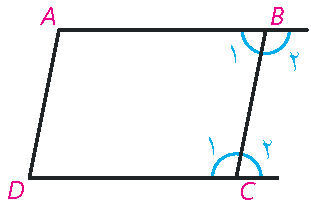
\includegraphics{"Shapes/Fasl - 3/Dars 1/qazie 2.pdf"}
	\end{flushleft}
\end{minipage}
\newline \bigskip \bigskip

\textbf{عکس قضیه ۲}: هر چهارضلعی که ر دو زاویه‌ی مجاور آن مکمل‌ باشند، متوازی‌الاضلاع است.

\begin{minipage}{.7\textwidth}
	\centering فرض: 
	$\left.
	\begin{array}{rrr}
		B_2 + D =180^{\circ} \\
		C_1 + D =180^{\circ} \\
		A + D = 180^{\circ} \\
		A + B_2 = 180^{\circ}
	\end{array}
	\right\}$
	\qquad حکم:
	$ \left. 
	\begin{array}{rrr}
		AB \parallel CD \\
		AD \parallel BC
	\end{array}
 \right\}$
	\begin{flushleft}
		$ \left.
		\begin{array}{rrr} 
			\widehat{C}_1 + \widehat{C}_2 = 180^{\circ} \\
			\widehat{C}_1 + \widehat{D} = 180^{\circ}
		\end{array}
	 \right\}
	  \rightarrow \widehat{D} = \widehat{C}_2 \Rightarrow AD \parallel BC$
	  
	  $\left.
	  \begin{array}{rrr} 
	  	\widehat{C}_1 + \widehat{B}_2 = 180^{\circ} \\
	  	\widehat{B}_1 + \widehat{B}_2 = 180^{\circ}
	  \end{array}
	  \right\}
	  \rightarrow \widehat{B}_1 = \widehat{C}_1 \Rightarrow AB \parallel CD$
	\end{flushleft}
\end{minipage}
\begin{minipage}{.3\textwidth}
	\begin{flushleft}
		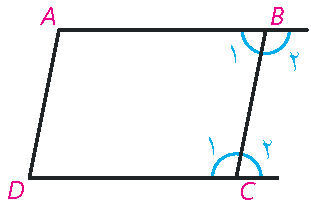
\includegraphics{"Shapes/Fasl - 3/Dars 1/qazie 2.pdf"}
	\end{flushleft}
\end{minipage}
\newline \bigskip \bigskip

\textbf{قضیه ۳}: در هر متوازی‌الضلاع، هر دو زاویه‌ی مقابل هم اندازه‌اند.

\begin{minipage}{.68\textwidth}
	\centering فرض: 
	$\left.
	\begin{array}{rrr}
		AB \parallel CD \\
		BC \parallel AD
	\end{array}
	\right\}$
	\qquad حکم:
	$ \left. 
	\begin{array}{rrr}
		\widehat{A} = \widehat{C} \\
		\widehat{B} = \widehat{D}
	\end{array}
 \right\}$
 \begin{flushright}
 	 بنا بر قضیه ۲ می‌توان نوشت:
 \end{flushright}
	\begin{flushleft}
		$ \left.
		\begin{array}{rrr} 
			\widehat{A} + \widehat{B} = 180^{\circ} \\
			\widehat{B} + \widehat{C} = 180^{\circ}
		\end{array}
	 \right\}
	 \rightarrow \widehat{A} = \widehat{C}
	 \qquad
	  \left.
	  \begin{array}{rrr} 
	  	\widehat{B} + \widehat{C} = 180^{\circ} \\
	  	\widehat{C} + \widehat{D} = 180^{\circ}
	  \end{array}
	  \right\}
	  \rightarrow \widehat{B} = \widehat{D}$
	\end{flushleft}
\end{minipage}
\begin{minipage}{.28\textwidth}
	\begin{flushleft}
		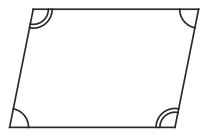
\includegraphics{"Shapes/Fasl - 3/Dars 1/qazie 3.pdf"}
	\end{flushleft}
\end{minipage}
\newline \bigskip \bigskip

\textbf{عکس قضیه ۳}: در هر یک چهارضلعی هر دو زاویه‌ی مقابل هم‌اندازه باشند، چهارضلعی متوازی‌الاضلاع است.

\begin{minipage}{.68\textwidth}
	\centering فرض: 
	$
		\widehat{A} = \widehat{C} = x \; , \; \widehat{B} = \widehat{C} = y
	$
	\qquad حکم:
	$ 
		ABCD 
	$ موازی‌الاضلاع است.
	\begin{flushleft}
		$ 
			x+y +x +y = 360^{\circ} \Rightarrow 2x + 2y = 360^{\circ} \Rightarrow x+y =180^{\circ}
		$
	\end{flushleft}
		هر دو زاویه‌ی مجاور مکمل‌اند،  بنابر عکس قضیه‌ ۲، ABCD متوازی‌الاضلاع است.
\end{minipage}
\begin{minipage}{.28\textwidth}
	\begin{flushleft}
		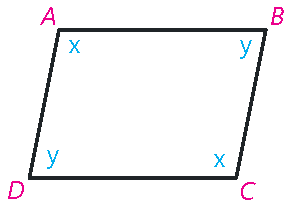
\includegraphics{"Shapes/Fasl - 3/Dars 1/qazie 3 ax.pdf"}
	\end{flushleft}
\end{minipage}
\newpage

\textbf{قضیه ۴}: در هر متوازی‌الاضلاع اقطار منصف یکدیگیرند.

\begin{minipage}{.68\textwidth}
	\centering فرض: 
	$
		AB \parallel CD \; , \; AD = BC
	$
	\qquad حکم:
	$ 
		OA = OC \; , \; OD = OB
	$
	\begin{flushleft}
		$ 
			\left. 
				\begin{array}{crr}
					\widehat{A}_1 = \widehat{C}_1 \\
					\widehat{B}_1 = \widehat{D}_1 \\
					AB = CD
				\end{array}
			\right\}
			\xRightarrow{\mbox{زض‌ز}} \triangle OAB \cong \triangle OCD \Rightarrow \left.
				\begin{array}{lll}
					OA = OC \\
					OB = OD
				\end{array}
			\right.
		$
	\end{flushleft}
\end{minipage}
\begin{minipage}{.28\textwidth}
	\begin{flushleft}
		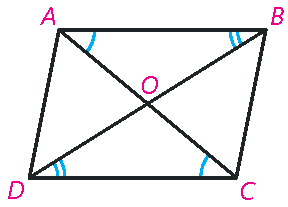
\includegraphics{"Shapes/Fasl - 3/Dars 1/qazie 4.pdf"}
	\end{flushleft}
\end{minipage}
\newline \bigskip \bigskip

\textbf{عکس قضیه ۴}: هر چهارضلعی‌ای که اقطارش منصف یکدیگر باشند، متوازی‌الاضلاع است.\\

\begin{minipage}{.68\textwidth}
	\centering فرض: 
	$
	 OA = OC \; , \; OD = OB
	$
	\qquad حکم:
	$ 
	AB \parallel CD \; , \; AD = BC
	$
	\begin{flushleft}
		$ 
		\left. 
		\begin{array}{crr}
			\widehat{O}_1 = \widehat{O}_2 \\
			OB = OD \\
			OA = OC
		\end{array}
		\right\}
		\xRightarrow{\mbox{ض‌زض}} \triangle OAB \cong \triangle OCD \Rightarrow \left.
		\begin{array}{cll}
			AB = CD \\
			\widehat{A}_1 = \widehat{C}_1 
		\end{array}
		\right.
		$
		$
		\widehat{A}_1 = \widehat{C}_1 \Rightarrow AB \parallel CD,\, \mbox{مورب} AC
		$
		
	\end{flushleft}
\end{minipage}
\begin{minipage}{.28\textwidth}
	\begin{flushleft}
		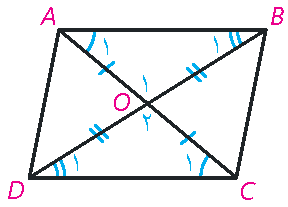
\includegraphics{"Shapes/Fasl - 3/Dars 1/qazie 4 ax.pdf"}
	\end{flushleft}
\end{minipage}
\newline \bigskip \bigskip

هر در چهارضلعی که دو ضلع آن هم‌اندازه و موازی باشند.، متوازی‌الاضلاع است.

\begin{minipage}{.68\textwidth}
	\centering فرض: 
	$
	AB = CD \; , \; AB \parallel CD
	$
	\qquad حکم:
	$ 
	BC \parallel AD
	$
	\begin{flushleft}
		$ 
		\left. 
		\begin{array}{crr}
			\widehat{A}_1 = \widehat{C}_1 \\
			AB = CD \\
			AC = AC
		\end{array}
		\right\}
		\xRightarrow{\mbox{ض‌زض}} \triangle ABC \cong \triangle ACD \Rightarrow
		\widehat{A}_2 = \widehat{C}_2 
		$
		$
		\widehat{A}_2 = \widehat{C}_2 \Rightarrow AD \parallel BC,\, \mbox{مورب} AC
		$
		
	\end{flushleft}
\end{minipage}
\begin{minipage}{.28\textwidth}
	\begin{flushleft}
		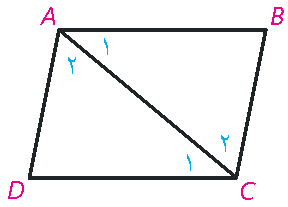
\includegraphics{"Shapes/Fasl - 3/Dars 1/2-1.pdf"}
	\end{flushleft}
\end{minipage}
\newline

\subsection{ویژگی‌هایی از مستطیل و لوزی}
در مستطیل 
$
ABCD
$،
دو قطر را رسم می‌کنیم. از هم‌نهشتی دو مثلث 
$
ACD
$
و
$
BCD
$
می‌توان نتیجه گرفت 
$
AC = BD
$.

\begin{minipage}{.68\textwidth}
	\begin{flushleft}
		$ 
		\left. 
		\begin{array}{crr}
			\widehat{D} = \widehat{C} \\
			AD = BC \\
			CD = CD
		\end{array}
		\right\}
		\xRightarrow{\mbox{ض‌زض}} \triangle ACD \cong \triangle BCD \Rightarrow
		AC = BD
		$
		
	\end{flushleft}
\end{minipage}
\begin{minipage}{.28\textwidth}
	\begin{flushleft}
		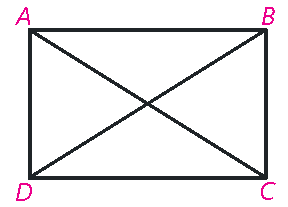
\includegraphics{"Shapes/Fasl - 3/Dars 1/2-1.1.pdf"}
	\end{flushleft}
\end{minipage}
\newline

بنابراین در هر مستطیل اقطار برابرند.

اگر دو قطر یک چهار ضلعی هم‌اندازه باشند. نمی‌توان نتیجه گرفت که آن چهارضلعی مستطیل است، ولی اگر آن چهارضلعی متوازی‌الاضلاع باشد، حتما مستطیل است.

\begin{minipage}{.47\textwidth}
	\begin{flushleft}
		$ 
		\left. 
		\begin{array}{crr}
			AC = BD \\
			AD = BC \\
			CD = CD
		\end{array}
		\right\}
		\xRightarrow{\mbox{ض‌ض‌ض}} \triangle ACD \cong \triangle BCD 
		$
		\centering
		$
		\rightarrow 
		\widehat{D} =\widehat{C} = 90^{\circ}
		$
		
	\end{flushleft}
\end{minipage}
\begin{minipage}{.49\textwidth}
	\begin{flushleft}
		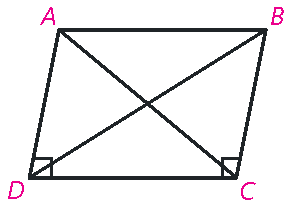
\includegraphics{"Shapes/Fasl - 3/Dars 1/2-1.3.pdf"}
		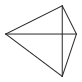
\includegraphics{"Shapes/Fasl - 3/Dars 1/2-1.2.pdf"}
	\end{flushleft}
\end{minipage}

\subsection{ویژگی‌ مهمی در مثلث قائم‌الزاویه}
در هر مثلث قائم‌الزاویه ‌اندازه‌ی میانه‌ی وارد بر وتر
 \textbf{نصف}
 اندازه‌ی وتر است.
 
 \begin{minipage}{.65\textwidth}
 	\centering فرض: 
 	$
 	\widehat{A} = 90^{\circ} \; , \; BM = MC
 	$
 	\qquad حکم:
 	$ 
 	AM = \dfrac{BC}{2}
 	$
 	\newline
 	
 	روی نیم‌خط $AM$ نقطه‌ی $D$ را چنان در نظر می‌گیریم که $DM = AM$.
 	\begin{flushleft}
 		$ 
	 		\left. 
		 		\begin{array}{crr}
		 			BM = CM \\
		 			AM = DM 
		 		\end{array}
	 		\right\}
	 		\Rightarrow \mbox{متوازی‌الاضلاع } ABCD \xRightarrow{\widehat{A} = 90^{\circ}} \mbox{مستطیل } ABCD
 		$

		$
			\Rightarrow AD = BC \Rightarrow
			BM = CM = AM = DM \Rightarrow AM = \dfrac{BC}{2}
		$

 	\end{flushleft}
 \end{minipage}
 \begin{minipage}{.28\textwidth}
 	\begin{flushleft}
 		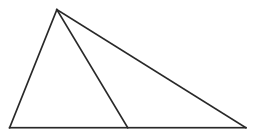
\includegraphics{"Shapes/Fasl - 3/Dars 1/2-2.1.pdf"}
 	\end{flushleft}
 \end{minipage}
 \newline \bigskip
 
 اگر در مثلثی اندازه‌ی میانه‌ی وارد بر ضلع، نصف اندازه‌ی آن ضلع باشد، آن مثلث قائم‌الزاویه‌ است.
 
  \begin{minipage}{.65\textwidth}
 	\centering فرض: 
 	$
 	 AM = \dfrac{BC}{2} \; , \; BM = CM
 	$
 	\qquad حکم:
 	$ 
 	\widehat{A} = 90^{\circ}
 	$
 	\newline
 	روی نیم‌خط $AM$ نقطه‌ی $D$ را چنان در نظر می‌گیریم که $DM = AM$.
 	\begin{flushleft}
 		$ 
	 		\left. 
		 		\begin{array}{crr}
		 			AM = \dfrac{BC}{2} \\
		 			\dfrac{AD}{2} = AM = DM
		 		\end{array}
	 		\right\}
	 		\Rightarrow \dfrac{BC}{2} = \dfrac{AD}{2} \Rightarrow BC =AM 
 		$
 		$
			\left. 
	 			\begin{array}{crr}
	 				\dfrac{AD}{2} =  AM = DM\\
	 				\dfrac{BC}{2} = BM = CM
	 			\end{array}
			\right\}
 			\Rightarrow AM = BM = CM = DM
 		$
 		$
 			\Rightarrow \mbox{مستطیل‌} ANCD \Rightarrow \widehat{A} = 90^{\circ}
 		$
 		
 	\end{flushleft}
 \end{minipage}
 \begin{minipage}{.34\textwidth}
 	\begin{flushleft}
 		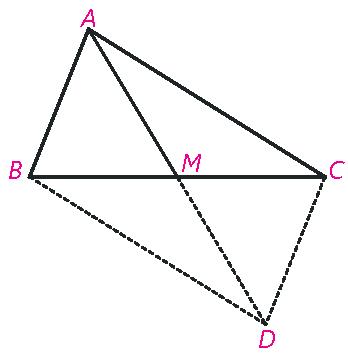
\includegraphics{"Shapes/Fasl - 3/Dars 1/2-2.2.pdf"}
 	\end{flushleft}
 \end{minipage}
 

\subsection{ویژگی‌هایی که فقط در لوزی برقرارند}

\begin{minipage}{.8\textwidth}
	اقطار لوزی
	$ABCD$
	را رسم می‌کنیم. چون لوزی متوازی‌الاضلاع است، اقطار منصف یکدیگرند. 
	$
	\triangle ABD
	$
	نیز متساوی‌الساقین است.
	
	نقطه تلاقی دو قطر را
	$H$
	می‌نامیم، در مثلث
	$ABD$،
	$AH$
	عمودمنصف
	$BD$
	و روی نیمساز 
	$
	\widehat{A}
	$
	است.
	
	بنابراین؛
	\newline \smallskip
	
	{\large در هر لوزی اقطار \textbf{عمودمنصف} یکدیگیر و روی \textbf{نیمساز} زوایا هستند.}
	
\end{minipage}
\begin{minipage}{.2\textwidth}
	\begin{flushleft}
		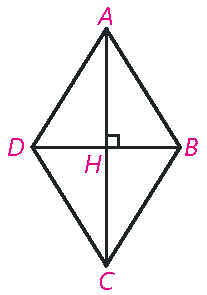
\includegraphics[width=3cm]{"Shapes/Fasl - 3/Dars 1/2-3.1.pdf"}
	\end{flushleft}
\end{minipage}
\newpage

\subsection{ذوزنقه}
ذوزنقه چهارضلعی‌ای است که با چهارضلعی‌هایی که قبلاً بررسی کردیم، کمی متفاوت است.

\textbf{تعریف:} ذوزنقه چهارضلعی‌ای است که فقط دو ضلع آن موازی باشند.

\begin{minipage}{.67\textwidth}

هر یک از دو ضلع $AB$، $CD$ را که موازی‌اند، \textbf{قاعده} و هر یک از دو ضلع غیر موازی را \textbf{ساق} می نامند. از موازی بودن قاعده‌های $AB$ ، $CD$ و قاطع‌های $BC$ و $AD$ در زوایا می‌توان نتیجه گرفت که:
\newline

زوایای $ \widehat{A}$ و $ \widehat{ِD}$ مکمل‌اند، همچنین زوایای  $ \widehat{B}$ و $ \widehat{C}$ مکمل هستند.
\newline

اگر در یک ذوزنقه یک ساق برابر باشند، آن را ذوزنقه متساوی‌الساقین می‌نامند.
\newline

هرگاه در یک ذوزنقه یک ساق بر قاعده‌ها عمود باشد، مسلماً بر قاعده‌ی دیگر نیز عمود است. در این صورت ذوزنقه را قائم‌الزاویه می‌نامند.
\end{minipage}
\begin{minipage}{.3\textwidth}
	\begin{center}
		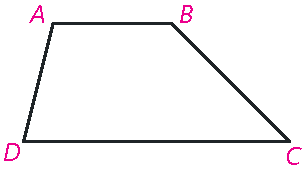
\includegraphics{"Shapes/Fasl - 3/Dars 1/2-4.1.pdf"}
		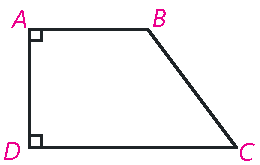
\includegraphics{"Shapes/Fasl - 3/Dars 1/2-4.2.pdf"}
	\end{center}
\end{minipage}

در هر ذوزنقه‌ی متساوی‌الساقین زاویه‌های مجاور به یک قاعده هم‌اندازه‌اند.

\begin{minipage}{.67\textwidth}
\begin{center}
	فرض:
	$
		\left.
			\begin{array}{ccc}
				AD = BC \\
				AB \parallel CD
			\end{array}
		\right\}
	$
	\qquad
	حکم:
	$
		\left.
			\begin{array}{ccc}
				\widehat{C} = \widehat{D} \\
				\widehat{A} = \widehat{B}
			\end{array}
		\right\}
	$
\end{center}
\begin{flushleft}
	$
	\left.
	\begin{array}{ccc}
		AD = BF \\
		AD = BC
	\end{array}
	\right\}
	\Rightarrow BF = BC  \rightarrow \widehat{E}_1 = \widehat{C}
	$
	
	$
	\left.
	\begin{array}{ccc}
		\widehat{E}_1 = \widehat{C} \\
		\widehat{E}_1 = \widehat{D}
	\end{array}
	\right\}
	\Rightarrow \widehat{C} = \widehat{D}
	$
\end{flushleft}
\end{minipage}
\begin{minipage}{.4\textwidth}
\begin{center}
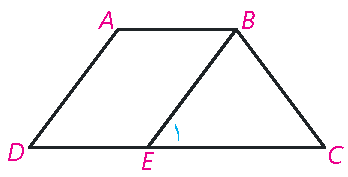
\includegraphics{"Shapes/Fasl - 3/Dars 1/2-4.3.pdf"}
\end{center}
\end{minipage}

اگر در یک ذوزنقه دو زاویه‌ی مجاور به یک قاعده هم‌اندازه باشند، ذوزنقه متساوی‌الساقین است.

\begin{minipage}{.67\textwidth}
	\begin{center}
		فرض:
		$
		\left.
		\begin{array}{ccc}
			\widehat{C} = \widehat{D} \\
			AB \parallel CD
		\end{array}
		\right\}
		$
		\qquad
		حکم:
		$
		\left.
		\begin{array}{ccc}
			 AD = BC 
		\end{array}
		\right\}
		$
	\end{center}
	\begin{flushleft}
		$
		\left.
		\begin{array}{ccc}
			\widehat{D} = \widehat{E}_1 \\
			\widehat{C} = \widehat{D}
		\end{array}
		\right\}
		\Rightarrow \widehat{E}_1 = \widehat{C} \rightarrow  BE = BC 
		$
		
		$
		\left.
		\begin{array}{ccc}
			 BF = BC  \\
			AD = BF
		\end{array}
		\right\}
		\Rightarrow AD = BC
		$
	\end{flushleft}
\end{minipage}
\begin{minipage}{.4\textwidth}
	\begin{center}
		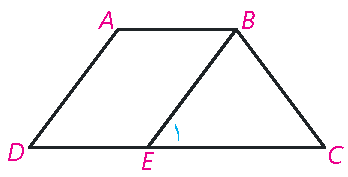
\includegraphics{"Shapes/Fasl - 3/Dars 1/2-4.3.pdf"}
	\end{center}
\end{minipage}

در هر ذوزنقه‌ی متساوی‌الساقین، اقطار اندازه‌های مساوی دارند و برعکس.
\smallskip

\begin{minipage}{.6\textwidth}
		فرض:
		$
		AB \parallel CD , AD = BC
		$
		\qquad
		حکم:
		$
		AC = BD
		$
	\begin{flushleft}
		$
		\left.
		\begin{array}{ccc}
			AD = BC \\
			CD = CD \\
			\widehat{C} = \widehat{D}
		\end{array}
		\right\}
		\xRightarrow{\mbox{ض‌زض}} \triangle BDC \equiv \triangle ADC \rightarrow  AC = BD 
		$
	\end{flushleft}
\end{minipage}
\begin{minipage}{.35\textwidth}
	\begin{center}
		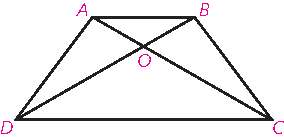
\includegraphics{"Shapes/Fasl - 3/Dars 1/PDFs/P63-S1.pdf"}
	\end{center}
\end{minipage}

\begin{minipage}{.6\textwidth}
		
		فرض:
		$
		AC = BD
		$
		\qquad
		حکم:
		$
		AD = BC
		$
	\begin{flushleft}
		$
		\left.
		\begin{array}{ccc}
			AH' = BH \\
			AC = BD 
		\end{array}
		\right\}
		\xRightarrow{\mbox{وض}} \triangle AH'C \cong \triangle BHD \rightarrow  D_1 = C_1 
		$
		\smallskip
		
		$
		\left.
		\begin{array}{ccc}
			D_1 = C_1 \\
			CD = CD  \\
			AC = BD
		\end{array}
		\right\}
		\xRightarrow{\mbox{ض‌زض}} \triangle ADC \cong \triangle ‌BDC \rightarrow  AD = BC
		$
	\end{flushleft}
\end{minipage}
\begin{minipage}{.35\textwidth}
	\begin{center}
		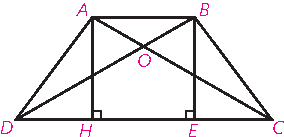
\includegraphics{"Shapes/Fasl - 3/Dars 1/PDFs/P63-S2.pdf"}
	\end{center}
\end{minipage}
\newpage

%\textbf{تمرین}
\subsection{تمرین}
	\subsubsection[1]{}
	۱ - در کدام n ضلعی تعداد اقطار و اضلاع برابر است؟
	\begin{flushleft}
		$
			n = \dfrac{n(n-3)}{2} \Rightarrow 2n = n^2 - 3n \Rightarrow n^2 -5n = 0 \Rightarrow n(n-5) = 0 \Rightarrow 
			\left\{
				\begin{array}{lll}
					x = 0 & \mbox{ق‌ق} \\
					\fbox{$x = 5$} &  \mbox{غ‌ق‌ق} 
				\end{array}
			\right.
		$
	\end{flushleft}
	\subsubsection[2]{}
		   \begin{minipage}{.75\textwidth}
	۲ - در دو چهارضلعی مقابل 
	 $ AB = A'B' $
	 و
	 $ \angle B = \angle B' $
	 و
	 $ BC = B'C' $
	 و
	 $ \angle C = \angle C' $
	 و
	 $ CD = C'D' $
	 است. چگونه مساوی بودن اندازه‌های سایر ضلع‌ها و زاویه‌ها را نتیجه می‌گیرید؟
	 \bigskip
	 
	 اگر 
	 $ \angle B = \angle B' $
	 و
	 $ BC = B'C' $
	 و
	 $ \angle C = \angle C' $
	 و
	 $ CD = C'D' $
	 و
	  $ \angle D = \angle D' $
	  در این حالت چگونه مساوی بودن اندازه‌های سایر ضلع‌ها و زاویه‌ها را نتیجه می‌گیرید؟
	  
	  \end{minipage}
	  \begin{minipage}{.25\textwidth}
	  	\begin{flushleft}
	  		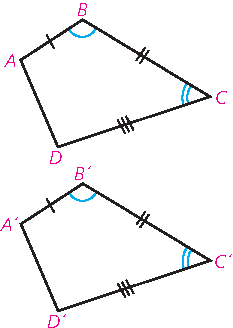
\includegraphics{"Shapes/Fasl - 3/Dars 1/PDFs/P63-S3,4.pdf"}
	  	\end{flushleft}
	  \end{minipage}
	  
	\subsubsection[3]{}
	    \begin{minipage}{.75\textwidth}
			
			۳ - از تقاطع نیم‌سازهای داخلی یک متوازی‌الضلاع، چهارضلعی
			$MNPQ$
			پدید آمده‌است. ثابت کنید این چهارضعلی مستطیل است.
	   \end{minipage}
	   \begin{minipage}{.25\textwidth}
	   	\begin{flushleft}
	   		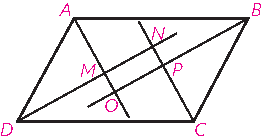
\includegraphics{"Shapes/Fasl - 3/Dars 1/PDFs/P63-S5.pdf"}
	   	\end{flushleft}
	   \end{minipage}
   
   	\begin{flushleft}
	$
   		\left.
   			\begin{array}{lll}
   				\widehat{B} = \widehat{C} = 180^{\circ} \Rightarrow 2 \alpha + 2 \beta =180^{\circ} \Rightarrow \alpha + \beta = 90^{\circ}  \Rightarrow \widehat{P}_1 = \widehat{P}_2 = 90^{\circ} \\
			   	\widehat{A} = \widehat{D} = 180^{\circ} \Rightarrow 2m + 2n =180^{\circ} \Rightarrow m + n = 90^{\circ}  \Rightarrow \widehat{M}_2 = \widehat{M}_1 = 90^{\circ} \\
			   	\widehat{C} = \widehat{D} = 180^{\circ} \Rightarrow 2 n + 2 \alpha =180^{\circ} \Rightarrow m + \alpha = 90^{\circ}  \Rightarrow \widehat{N}_1 = \widehat{N}_2 = 90^{\circ}  \\
	   	   		\widehat{P}_2 + \widehat{M}_1 + \widehat{N}_2 + \widehat{Q}_2= 360^{\circ} \Rightarrow 270^{\circ} + \widehat{Q}_2 = 360^{\circ} \Rightarrow \widehat{Q}_2 = 90^{\circ} 
   			\end{array}
   		\right\}
   		\Rightarrow \mbox{$MNPQ$ مستطیل}
   	$
   \end{flushleft}
   
	\subsubsection[4]{}
	 ۴ - مثلث قائم الزاویه‌ی 
	$\triangle ABC$
	  را که در آن 
	$\angle A$
	   قائمه و اندازه‌ی
	$\angle C$
	    برابر 
	$30^{\circ}$
	     است، در نظر می‌گیریم. میانه‌ی وارد بر وتر را رسم کنید. مثلث های 
	$AMC$
	و
	$AMB$
	 چگونه مثلث‌هایی هستند؟ نشان دهید 
	$AB = \dfrac{BC}{2}$
	  یعنی در هر مثلث قائم الزاویه اگر اندازه‌ی یک زاویه 
	$30^{\circ}$
	   باشد، اندازه‌ی ضلع مقابل آن نصف اندازه‌ی وتر است.
	 
	 سپس با استفاده از قضیه‌ی فیثاغورث نشان دهید
	$AC = \frac{\sqrt{3}}{2}BC$  
	 
	 یعنی در هر مثلث قائم الزاویه اگر یک زاویه 
	$60^{\circ}$
	  باشد، اندازه‌ی ضلع مقابل آن  اندازه‌ی وتر است.
	 
	 اکنون مثلث قائم الزاویه ای رسم کنید که اندازه‌ی یک زاویه‌ی آن 
	 $45^{\circ}$
	  باشد و نشان دهید که اندازه‌ی هر ضلع زاویه‌ی قائمه در آن 
	  $\frac{\sqrt{2}}{2}$
	   اندازه‌ی وتر است.
	   
		\begin{minipage}{.75\textwidth}
			\begin{flushleft}
					$
					BM = AM \Rightarrow \text{ABM متساوی‌الاضلاع است}
				$
				$
					CM = AM \Rightarrow \text{ACM متساوی‌الضاقین است}
				$
				$
					AB = \dfrac{BC}{2} \Rightarrow AB =MB = \dfrac{BC}{2}
				$
				
				$
					AB^2 + AC^2 = BC^2 \Rightarrow \dfrac{BC^2}{4} + AC^2 = BC^2 \Rightarrow AC^2 = BC^2 - \dfrac{BC^2}{4} \Rightarrow AC^2 = 3bc^2 \Rightarrow AC = BC \dfrac{\sqrt{3}}{2}
				$
			\end{flushleft}
		\end{minipage}
		\begin{minipage}{.25\textwidth}
		  	\begin{flushleft}
		  		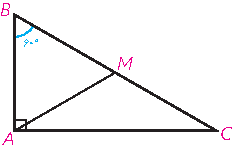
\includegraphics{"Shapes/Fasl - 3/Dars 1/PDFs/P64-S1.pdf"}
		  	\end{flushleft}
		\end{minipage}

	\subsubsection[5]{}
	 ۵ - در مثلث قائم الزاویه‌ی 
	 $\triangle ABC$
	  اندازه‌ی زاویه‌ی 
	  $\widehat{B}$
	   برابر 
	   $15^{\circ}$
	    است. با رسم میانه و ارتفاع وارد بر وتر نشان دهید اندازه‌ ارتفاع وارد بر وتر 
	    $\frac14$
	     اندازه‌ی وتر است.
	     
	  \begin{minipage}{0.75\textwidth}
	     	\begin{flushleft}
	     		$ \triangle AHM:$
	     		$
	     			\left.
		     			\begin{array}{ccc}
		     			    &	\widehat{M} = \left. 30^{\circ} \right\} \rightarrow & AH = \frac12 AM \\
		     				& &AM = \frac12 BC
		     			\end{array}
	     			\right\}
	     			\rightarrow AH = \frac12 \left( \frac12 BC \right) \Rightarrow AH = \frac14 BC
	     		$
	     	\end{flushleft}
	  \end{minipage}   
	\begin{minipage}{.25\textwidth}
		\begin{flushleft}
			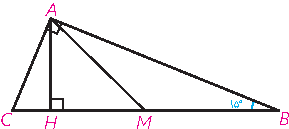
\includegraphics{"Shapes/Fasl - 3/Dars 1/PDFs/P64-S2.pdf"}
		\end{flushleft}
	\end{minipage}

	\subsubsection[6]{}
	 ۶ - در متوازی الاضلاع  
	 $ABCD$،
	 $M$ و $N$
	  به ترتیب وسط های ضلع های 
	  $AD$ و $BC$
	   می‌باشند. چرا خطوط
	   $MB$ و $ND$
	   موازی‌اند؟ به کمک آن ثابت کنید $AP = PQ = QC$
	\subsubsection[7]{}
7 - ثابت کنید اگر وسط های ضل عهای هر چهارضلعی را به طور متوالی به هم وصل کنیم، یک متواز یالاضلاع پدید می آید.
 
 این چهارضلعی باید چه ویژگی ای داشت هباشد تا این متواز یالاضلاع مستطیل یا لوزی شود؟
 
 چه رابطه ای بین محیط متوازی الاضلاع پدید آمده با انداز ههای قطر های چهارضلعی اولیه وجود دارد؟


\section{مساحت و کاربردهای آن}

یادآوری

١- اگر اندازهٔ یک ضلع مربع $a$ باشد، $S=a^2$ مساحت آن است.

۲- اگر اندازهٔ یک ضلع مثلث $a$ و اندازهٔ ارتفاع نظیر آن ضلع $h_a$ باشد، آنگاه $S = \frac12 ah_a$

بنابراین در هر مثلث ABC اگر اندازه‌ی اضلاع BC، AC و AB را به ترتیب با a، b و c اندازه‌های ارتفاع های نظیر آنها را به ترتیب با $h_a$، $h_b$ و $h_c$ شان دهیم آن‌گاه، $2S = ah_a = bh_b = ch_c$

۳- اگر اندازهٔ یک ضلع متوازی الاضلاع a و اندازهٔ ارتفاع نظیر آن h باشد، $S=ah$.

۴- اگر اندازه های دو قطر لوزی m و n باشند، $S=\frac12 nm$.

۵- اگر اندازه های دو قاعدهٔ یک ذوزنقه a و b و اندازه‌ی ارتفاع آن h باشد $S = \dfrac{(a+b)h}2$
\bigskip

\textbf{کار در کلاس}

فرض کنیم اندازهٔ هر ضلع مثلث متساوی الاضلاع ABC برابر a باشد، ارتفاع AH را رسم کنید. ارتفاع AH میانه نیز است؛ چرا؟

به کمک قضیهٔ فیثاغورس نشان دهید 
$AH = \dfrac{a\sqrt{3}}2$
و 
$S = \dfrac{a^2 \sqrt{3}}{4}$.
\bigskip

\textbf{فعالیت}

در چهارضلعی ABCD دو قطر AC و DB برهم عموداند.

با جمع این دو مساحت داریم:

$S_{ABCD} = \frac12 BD (AH + BH) = \frac12 BD \times AC$

بنابراین؛

\textbf{در هر چهارضلعی‌ای که دو قطر آن برهم عمود باشند، مساحت برابر است با نصف حاصل ضرب دو قطر. }

\subsection{کاربردهایی از مساحت}
قبلاً با کاربرد مساحت در اثبات قضیهٔ تالس آشنا شدید. بعضی رابطه ها و ویژگی‌هایی را که با آن آشنا شده اید یادآوری می کنیم.
\bigskip

\textbf{ویژگی ۱}:
در دو مثلث اگر اندازۀ قاعده‌ها برابر باشند، نسبت مساحت‌ها برابر نسبت اندازه‌ی ارتفاع‌های متناظر این قاعده‌هاست.
$
	\dfrac{S}{S'} = \dfrac{h}{h'}
$
\bigskip



\chapter{تجسم فضایی}

\section{خط، نقطه و صفحه}

\section{تفکر تجسمی}
	
\end{document}